\documentclass{beamer}
%
% Choose how your presentation looks.
%
% For more themes, color themes and font themes, see:
% http://deic.uab.es/~iblanes/beamer_gallery/index_by_theme.html
%
\mode<presentation>
{
  \usetheme{Szeged}      % or try Darmstadt, Madrid, Warsaw, ...
  \usecolortheme{beaver} % or try albatross, beaver, crane, ...
  \usefonttheme{professionalfonts}  % or try serif, structurebold, ...
  \setbeamertemplate{navigation symbols}{}
  \setbeamertemplate{caption}[numbered]
} 

\usepackage[english]{babel}
\usepackage[utf8x]{inputenc}
\usepackage{graphicx}
\usepackage{svg}
\usepackage{amsmath}
\usepackage{booktabs}
\usepackage{algorithm}
\usepackage{algpseudocode}
\usepackage{hyperref}
\usepackage{tikz}
\usetikzlibrary{positioning,angles,quotes}
\usetikzlibrary{arrows,shapes}
\usepackage{caption}
\usepackage{media9}

\everymath{\displaystyle}
\DeclareMathOperator*{\argmin}{arg\,min}
\DeclareMathOperator*{\argmax}{arg\,max}

\title[Data efficient reinforcement learning]{Data efficient reinforcement learning\\Gaussian process, PILCO and DeepPILCO}
\author{Ali Younes}
\institute[BMSTU]
{
  Bauman Moscow State Technical University \\ % Your institution for the title page
  \medskip
  \textit{ay20-5-1994@hotmail.com} % Your email address
}
\date{\today}

\begin{document}

\begin{frame}
  \titlepage
\end{frame}

% Uncomment these lines for an automatically generated outline.
\begin{frame}{Outline}
  \tableofcontents
\end{frame}

\section{Introduction}
\subsection{Data efficient reinforcement learning}
\begin{frame}{Why data efficient reinforcement learning?}
\begin{itemize}
  \item Reinforcement learning is a hot research topic nowadays.\\
  It is considered one of the major research directions in robot learning.
  \item We have worked with model free algorithms (TRPO, PPO).
\end{itemize}
  \begin{center}
  \captionsetup{labelformat=empty}
  \captionof{figure}{Reinforcement learning}
    \tikzstyle{block} = [rectangle, draw, 
    text width=7em, text centered, rounded corners, minimum height=3em]
    \tikzstyle{line} = [draw, -latex]
    \begin{tikzpicture}[node distance = 6em, auto, thick]
        \node [block] (Agent) {Agent};
        \node [block, below of=Agent] (Environment) {Environment};
        \path [line] (Agent.0) --++ (4em,0em) |- node [near start,align=center]{Action \\ $a_t$} (Environment.0);
        \path [line] (Environment.180) --++ (-4em,0em) |- node [near start,align=center] {State \\ $s_{t+1}$ \\Reward \\$r_{t+1}$} (Agent.180);
    \end{tikzpicture}
\end{center}{}
\end{frame}

\begin{frame}
  \frametitle{Why data efficient reinforcement learning?}
  \begin{figure}[h]
      \centering
      \captionsetup{labelformat=empty}
      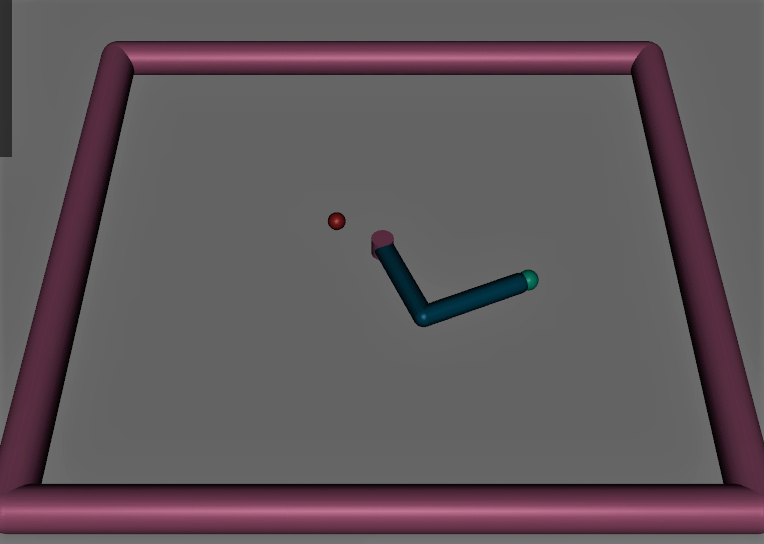
\includegraphics[height=6cm]{img/Reacher(Mujoco).png}
      \label{fig:my_label}
  \end{figure}
\end{frame}

\begin{frame}
  \frametitle{Why data efficient reinforcement learning?}
  \begin{figure}[h]
      \centering
      \captionsetup{labelformat=empty}
      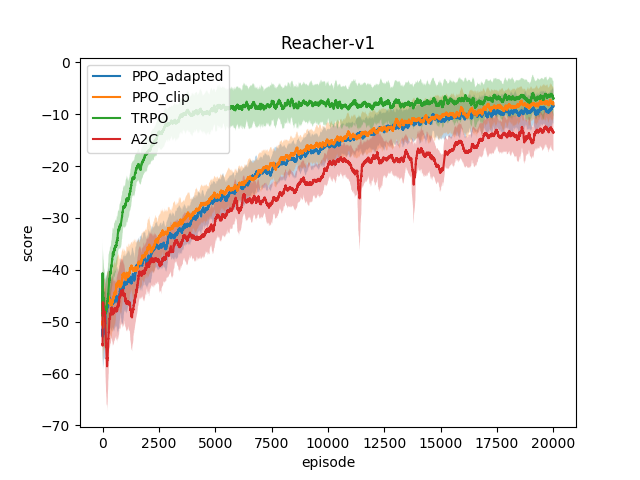
\includegraphics[height=7cm]{img/Reacher.png}
      \label{fig:my_label}
  \end{figure}
\end{frame}



\begin{frame}{Why data efficient reinforcement learning?}
\begin{itemize}
    \item In real world that means weeks of training.\\
    \textcolor{red}{Collecting samples is expensive in real world robots}
    \item We need a robot learning framework with as less as possible interaction time in the real world.\\
    Two solution:
    \begin{enumerate}
        \item Transfer learning from simulation to real world (Sim2Real)
        \item Data efficient learning
    \end{enumerate}
\end{itemize}
\end{frame}

\subsection{Gaussian Processes in RL}
\begin{frame}
  \frametitle{Model Based reinforcement learning}
\begin{center}
 \captionsetup{labelformat=empty}
 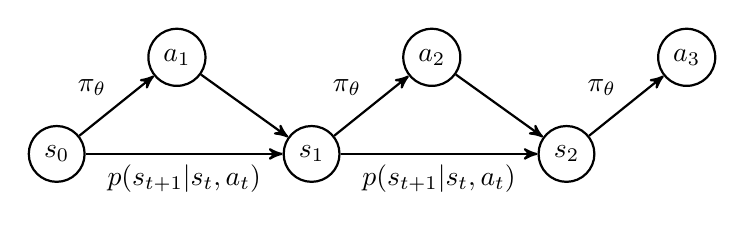
\begin{tikzpicture}[->, >=stealth', auto, thick, node distance=3cm]

    \tikzstyle{round}=[thick,draw=black,circle]

    \node[round] (s0) {$s_0$};
    \node[round,right= 25mm of s0] (s1) {$s_1$};
    \node[round,above right=7mm and 10mm of s0] (a1){$a_1$};
    \node[round,right= 25mm of s1] (s2) {$s_2$};
    \node[round,above right=7mm and 10mm of s1] (a2){$a_2$};
    \node[round,above right=7mm and 10mm of s2] (a3){$a_3$};

    \path (s0) edge node[below] {$p(s_{t+1}|s_t,a_t)$}(s1)
          (s0) edge node {$\pi_\theta$} (a1)
          (a1) edge node {} (s1);
    \path (s1) edge node[below] {$p(s_{t+1}|s_t,a_t)$}(s2)
          (s1) edge node {$\pi_\theta$} (a2)
          (a2) edge node {} (s2);
    \path (s2) edge node {$\pi_\theta$} (a3);
\end{tikzpicture}
\end{center}
\begin{itemize}
    \item We will use the following terminology:\\
    State : $x_t$ , Control (action): $u_t$ , Cost (reward): $c$
    \item Transition function: $x_{t+1}=f(x,u_t)+\omega$
    \item Control: $u_t=\pi (x_t,\theta )$
    \item The expected long-term cost:  $J(\theta)=\sum_{t=1}^{T} \mathbb{E} [c(x_t)|\theta]$
\end{itemize}
\end{frame}

\begin{frame}
	\frametitle{Gaussian processes}
    \begin{itemize}
    \item In probability theory and statistics, a Gaussian process is a stochastic process (a collection of random variables indexed by time or space), such that every finite collection of those random variables has a multivariate normal distribution, i.e. every finite linear combination of them is normally distributed.
    \item In other words, a  Gaussian process is a probability distribution over possible functions.
    \item Gaussian process defined by:
    \begin{enumerate}
        \item Mean function $m(.)$
        \item Covariance function (Kernel) $k(.,.)$
    \end{enumerate}
    \end{itemize}
\end{frame}

\begin{frame}{Gaussian processes - Regression}
\begin{center}
    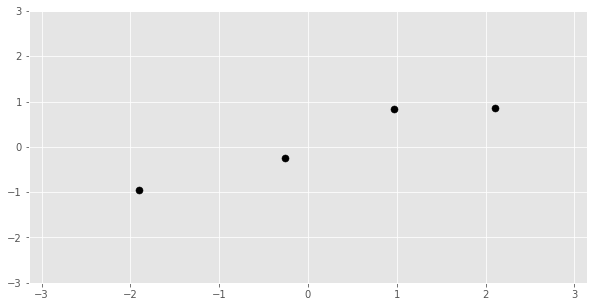
\includegraphics[height=3cm]{img/data.png}
    
    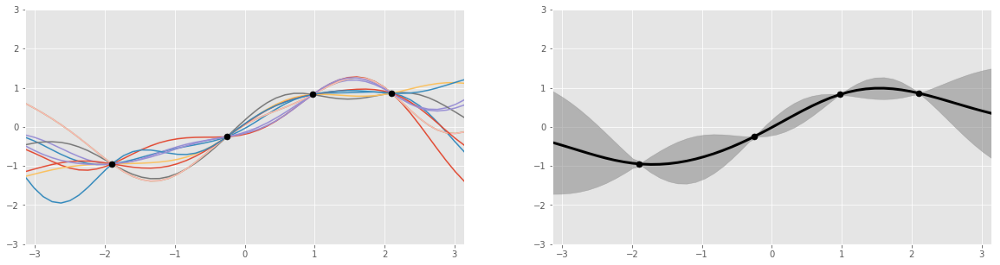
\includegraphics[height=3cm]{img/DPregression.png}
\end{center}
\end{frame}

\section{PILCO}

\subsection{PILCO Algorithm}

\begin{frame}
  \frametitle{PILCO Algorithm}
  \begin{itemize}
  \item 
  M. Deisenroth and C. Rasmussen, \\
  “PILCO: A model-based and data-efficient approach to policy search”,ICML-2011\\
  M. Deisenroth, D. Fox, and C. Rasmussen,\\
  “Gaussian processes for data-efficient learning in robotics and control", PAMI-2015
  \item PILCO (Probabilistic Inference for Learning COntrol)
  \item A model based policy search method, considering the model uncertainty while learning models. PILCO Uses Gaussian processes as a probabilistic model.
  \end{itemize}
\end{frame}

\begin{frame}
\frametitle{PILCO Algorithm: High-level steps}
\begin{enumerate}
    \item Probabilistic model for transition function f \\
     (system identification)
    \item Compute long-term predictions $p(x_1|\theta),....,p(x_T|\theta)$
    \item Policy improvement
    \item Apply controller
\end{enumerate}
\end{frame}

\subsection{PILCO Algorithm components}
\begin{frame}{1. Model Learning (System Identification)}
    Model learning problem: Find a function $f:x \mapsto f(x)=y$
    \begin{center}
        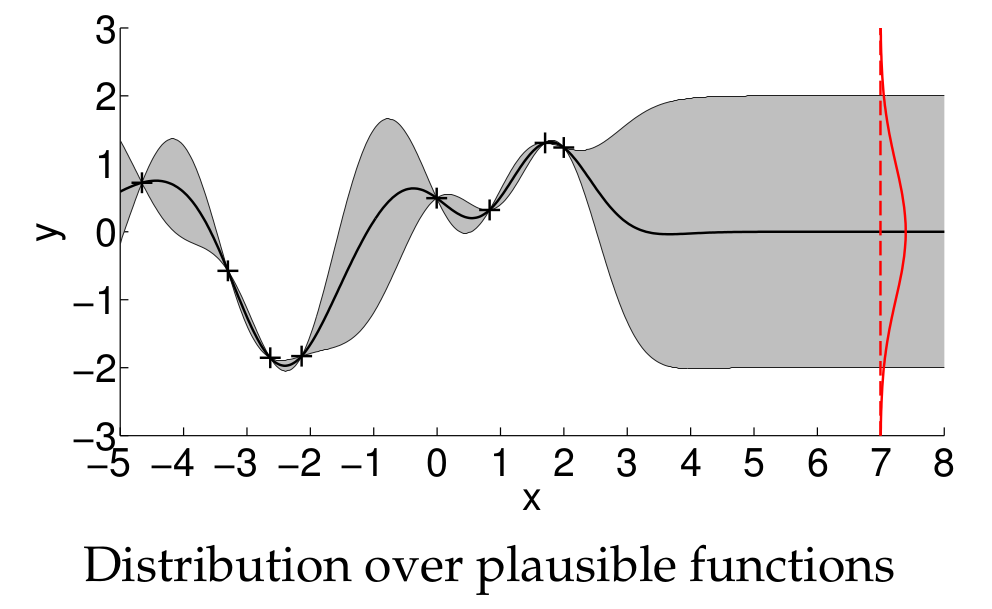
\includegraphics[height=4cm]{img/modellearning.png}
    \end{center}
    Express uncertainty about the underlying function to be robust to model errors. Posterior GP prediction $p(x_{t+1}|x_t,u_t)$
\end{frame}

\begin{frame}{2. Long-Term Predictions (Policy evaluation)}
    \begin{center}
        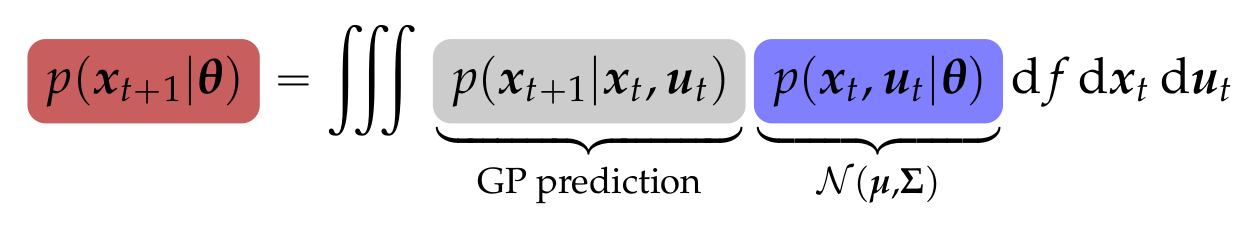
\includegraphics[height=1.8cm]{img/ltd-eq.png}\\
        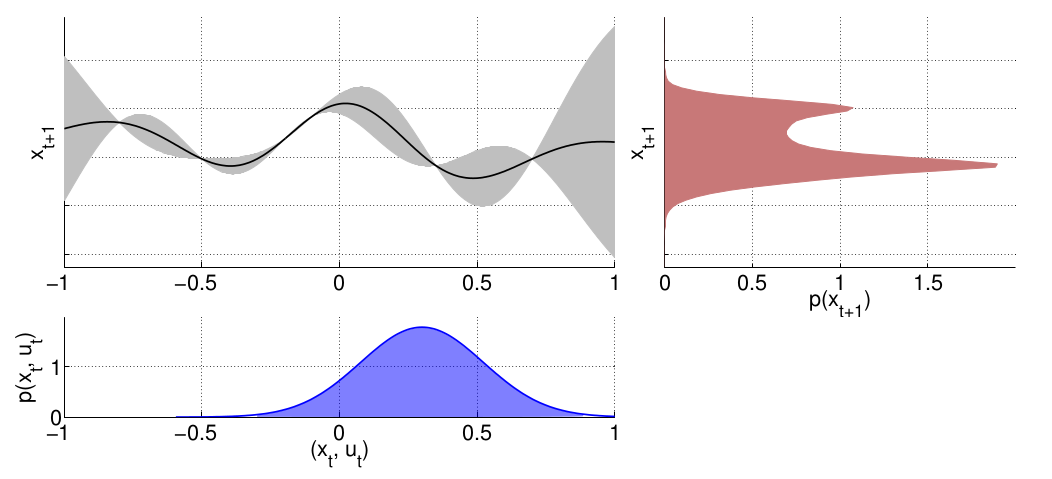
\includegraphics[height=5cm]{img/ltp.png}
    \end{center}
\end{frame}

\begin{frame}{2. Long-Term Predictions (Policy evaluation)}
Approximating $p(x_t+1)$ (red in the last image) by a Gaussian.\\
Using : 1. linearization of the posterior mean function
\begin{center}
    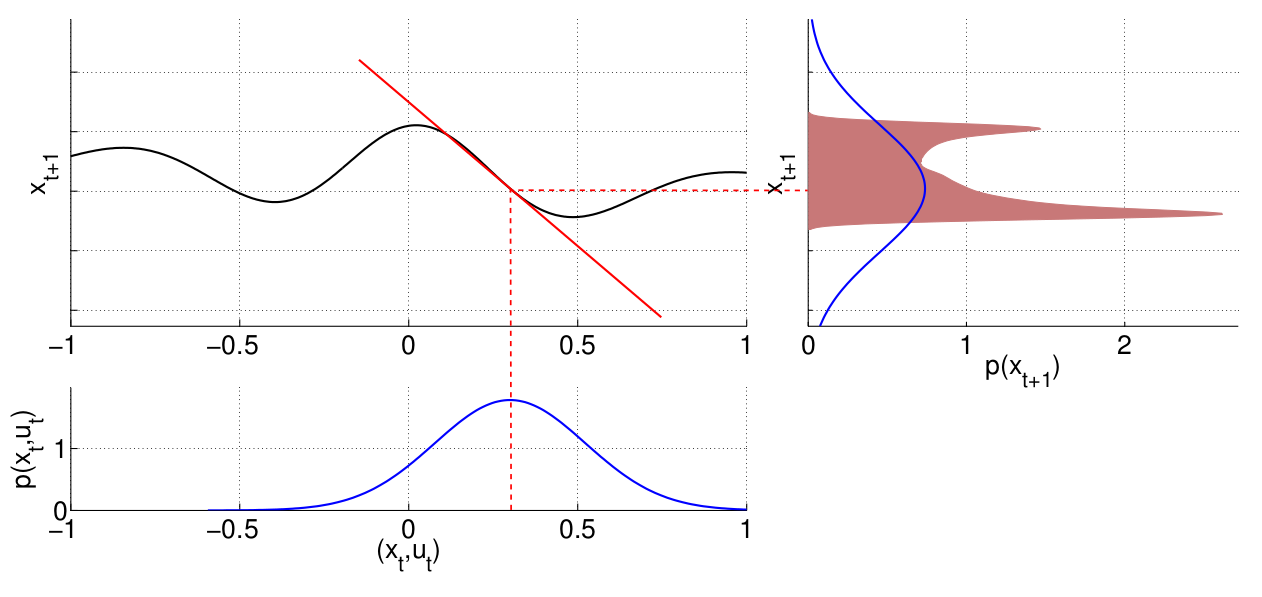
\includegraphics[height=5cm]{img/lin.png}
\end{center}
\end{frame}

\begin{frame}{2. Long-Term Predictions (Policy evaluation)}
Approximating $p(x_t+1)$ (red in the last image) by a Gaussian.\\
Using : 2. Moment matching
\begin{center}
    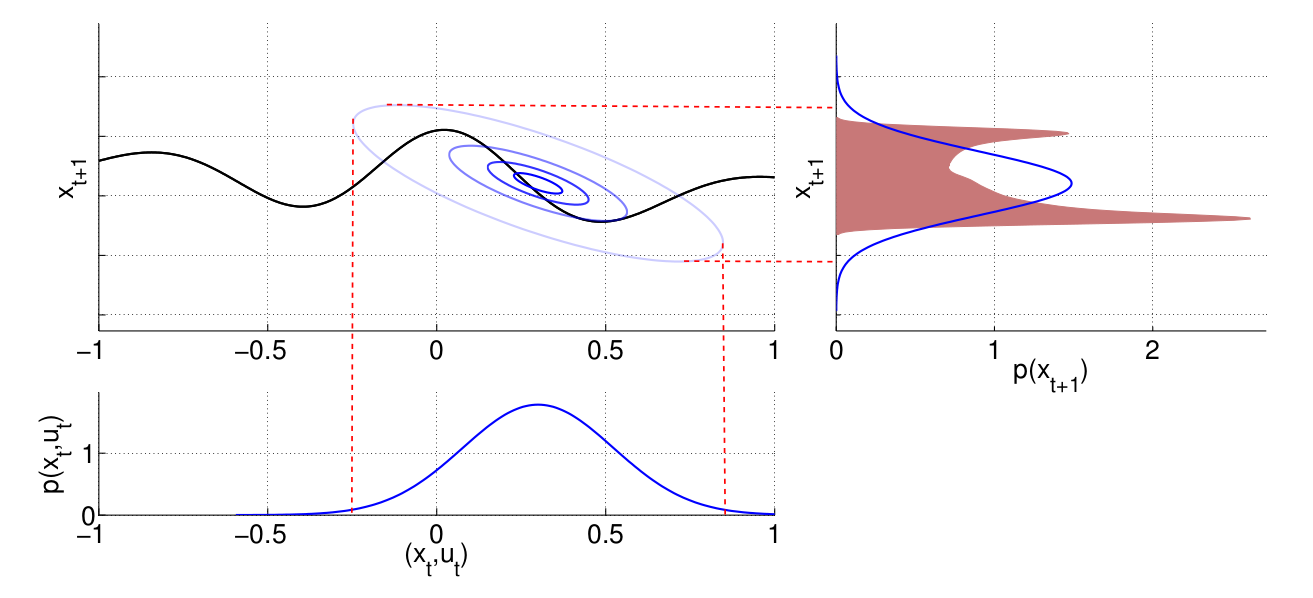
\includegraphics[height=5cm]{img/mom.png}
\end{center}
\end{frame}

\begin{frame}{2. Long-Term Predictions (Policy evaluation)}
To evaluate expected long term cost $J(\theta)$ we choose cost function $c$ such that inner the integral can be computed \textcolor{red}{analytically}:
$$J(\theta)=\sum_{t=1}^{T} \mathbb{E} [c(x_t)|\theta]=\sum_{t=1}^{T} \int c(x_t) \mathcal{N}(x_t|\mu_t,\Sigma_t) dx_t$$
\end{frame}

\begin{frame}{3. Policy Improvement and 4. Apply controller}
\begin{itemize}
    \item Analytically compute $\frac{d J^\pi (\theta)}{d\theta}$ for a gradient based policy search.
    \item We use standard gradient based optimizer (e.g. BFGS) to compute $\theta^*$
    \item Apply controller
\end{itemize}
\end{frame}

\subsection{Experimental results}
\begin{center}
Learning to Control a Low-Cost Manipulator\\
    \href{https://www.youtube.com/watch?v=gdT6dwUOYC0}{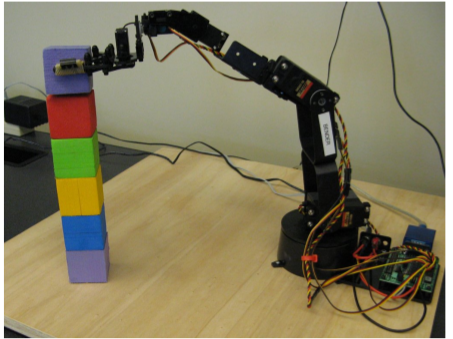
\includegraphics[height=7cm]{img/arm-p.png}}
\end{center}

\subsection{Experimental results}
\begin{center}
Learning to Control a Low-Cost Manipulator
    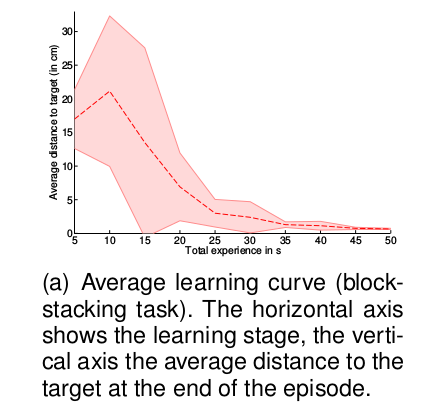
\includegraphics[height=6.5cm]{img/curve-arm.png}
\end{center}

\section{Deep PILCO}
\subsection{PILCO problems}
\begin{frame}{PILCO algorithm}
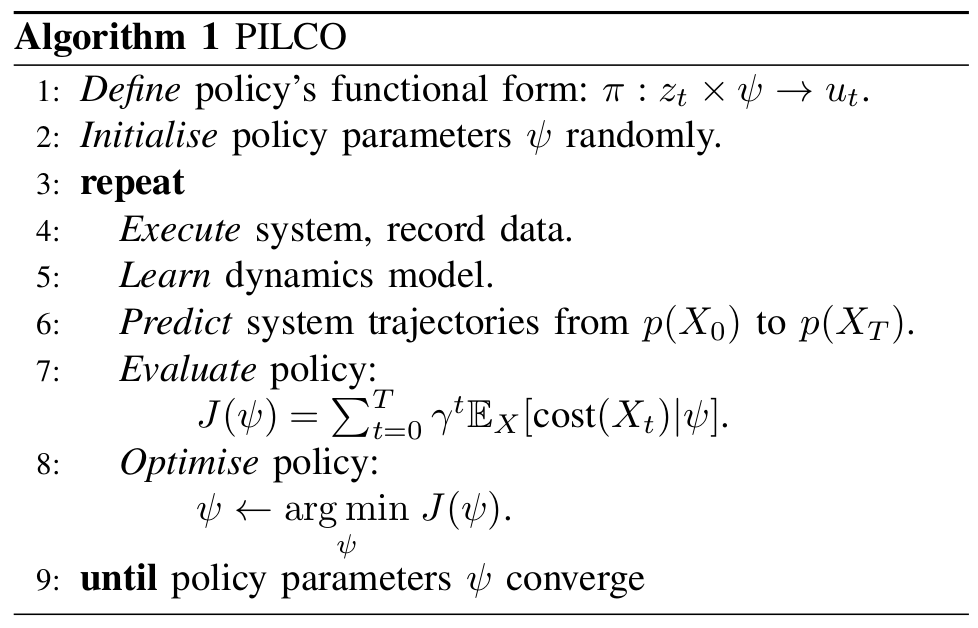
\includegraphics[height=7cm]{img/pilco-algo.png}
\end{frame}
\begin{frame}{PILCO problems}
    \begin{itemize}
        \item PILCO relies on Gaussian processes, which work extremely will with small amount of low dimentional data, but \textbf{scale cubically} with the number of trials, so PILCO is hard to scale to high dimensional observation spaces.
        \item PILCO doesn't consider temporal correclation between successive state transitions. This means that PILCO \textbf{underestimates state uncertainty at future time steps.} which can lead to diminished performance.
    \end{itemize}
\end{frame}
\begin{frame}{Deep PILCO}
    \begin{itemize}
        \item Deep PILCO (Improving  PILCO  with  Bayesian  Neural  Network  Dynamics  Models)\\
        (Yarin Gal and Rowan Thomas McAllister and Carl Edward Rasmussen - 2016)
        \item DeepPILCO : \\
        Gaussian processes $\rightarrow$ Bayesian deep dynamic model
    \end{itemize}
\end{frame}
\begin{frame}{Deep PILCO idea}
\begin{itemize}
    \item Deep PILCO uses deep neural network capable of scaling to high dimensional observation spaces.
    \item The dynamic model that rely on DNN should maintain the probabilistic nature of the GP, capturing :
    \begin{enumerate}
        \item Output uncertainty
        \item Input uncertainty
    \end{enumerate}
\end{itemize}
\end{frame}
\begin{frame}{1. Output uncertainty solution}
\begin{itemize}
    \item Simple NN models cannot express output model uncertainty.
    \item Using Bayesian probabilistic equivalent to the NN -\\ the \textbf{Bayesian neural network (BNN)}
    \item Represent the model uncertainty with an \textbf{approximate} posterior distribution over the weights of the BNN.
    \item \textbf{Dropout} can be interpreted as a variational Bayesian approximation. and can be used to approximate posterior distribution.
    \item Uncertainty in weights induces prediction uncertainty.
\end{itemize}
\end{frame}

\begin{frame}{1. Output uncertainty solution - Dropout}
    \begin{center}
        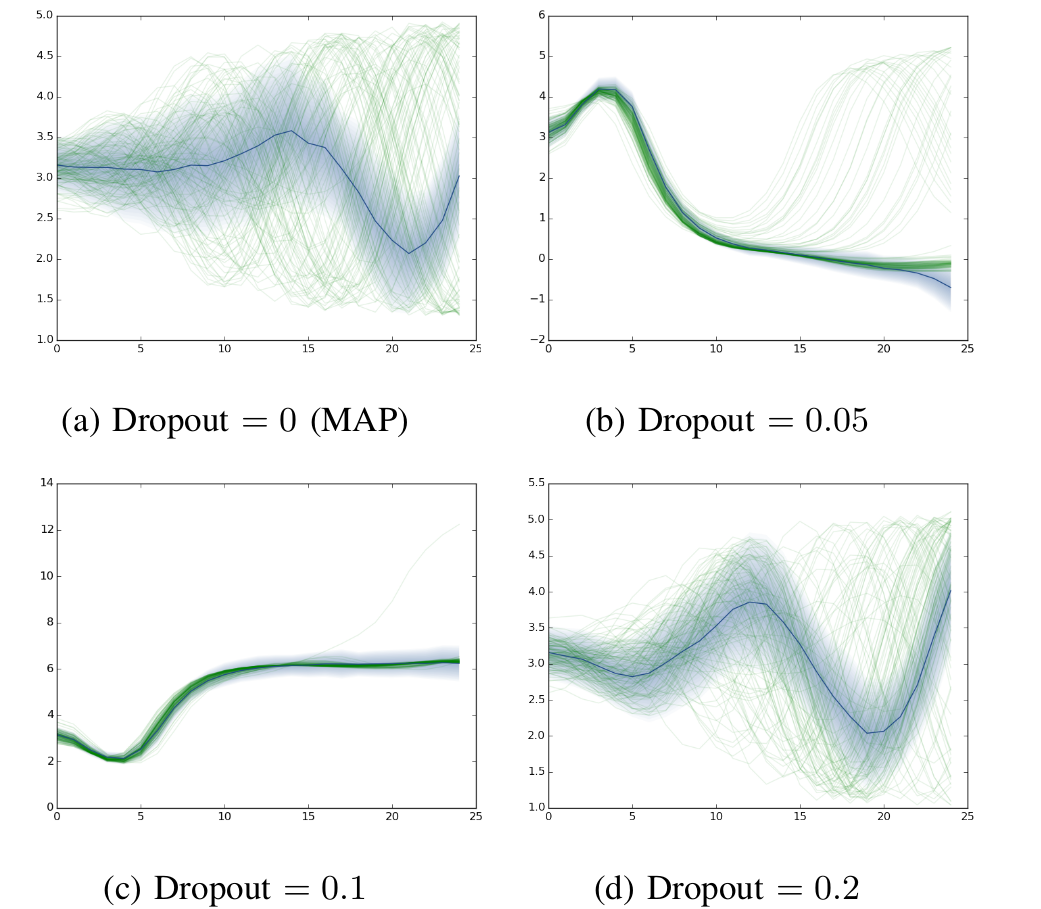
\includegraphics[height=6.5cm]{img/dropout.png}
    \end{center}
\end{frame}

\begin{frame}{2. Input uncertainty solution}
\begin{itemize}
    \item Handle input uncertainty = plan under dynamic uncertainty.\\
          Predict system trajectories from $p(x_0)$ to $p(x_T)$
    \item PILCO propagates state distributions through the dynamic model (GP) analytically, which cannot be done with NNs.
    \item The solution for this problem was using \textbf{particle methods}.
    \items Moment matching the output distribution at each time step, is used to forcing unimodal fit, where the algorithm penalizes policies that cause the predictive state to bifurcate.
\end{itemize}
\end{frame}

\begin{frame}{2. Input uncertainty solution - Particle method}
\begin{center}
    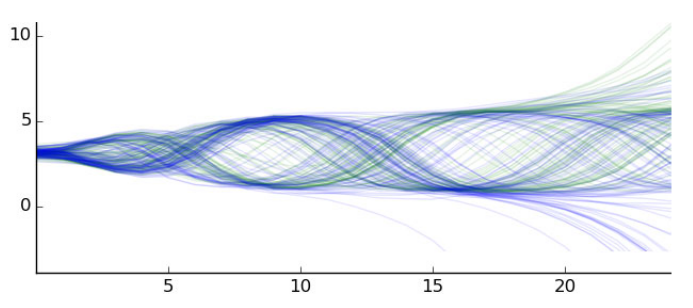
\includegraphics[width=\textwidth]{img/particles.png}
\end{center}
\end{frame}

\begin{frame}{PILCO algorithm}
    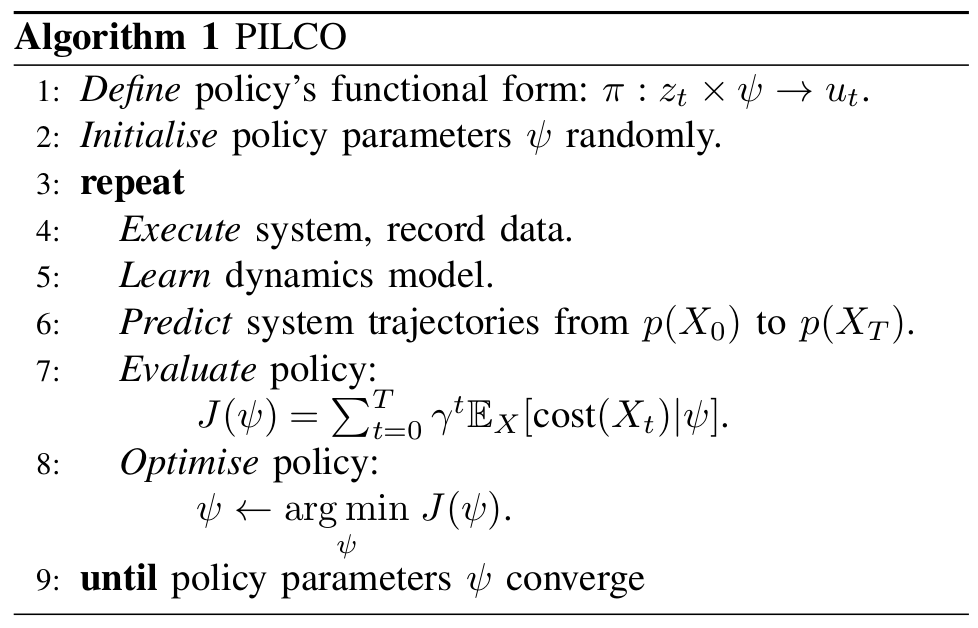
\includegraphics[height=7cm]{img/pilco-algo.png}
\end{frame}

\begin{frame}{DeepPILCO modification}
    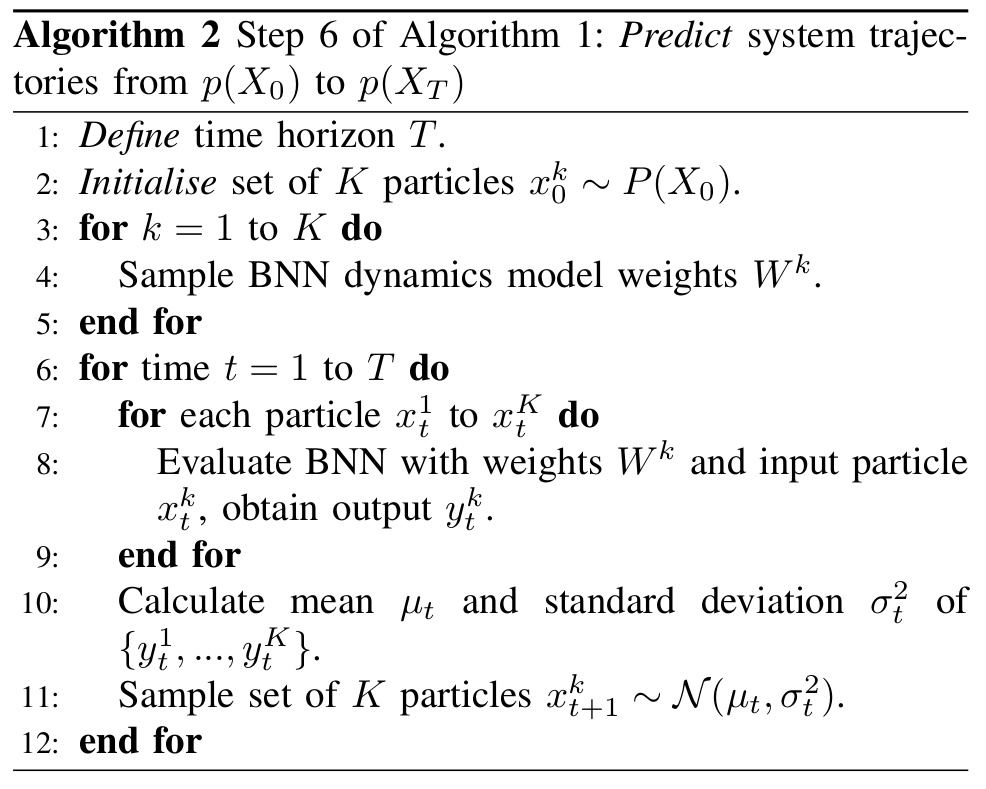
\includegraphics[height=7cm]{img/deep-algo.png}
\end{frame}

\begin{frame}{DeepPILCO results on cartpole}
    \begin{center}
        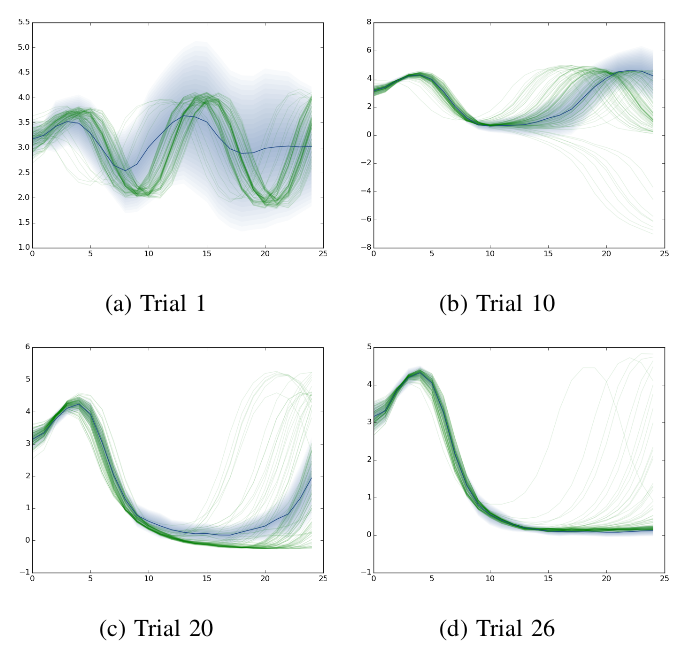
\includegraphics[height=6.5cm]{img/deep-curve.png}
    \end{center}
\end{frame}

\begin{frame}{Results continued}
\begin{itemize}
    \item DeepPILCO as a Bayesian approach to data efficient deep RL.
    \item Comparing DeepPILCO to DDPG and NAF (Normalized Advantage Functions)
\end{itemize}
    
    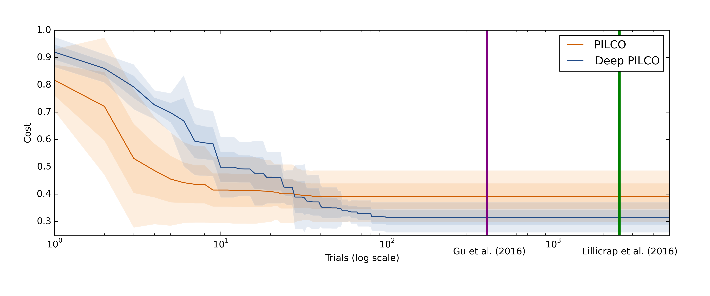
\includegraphics[width=\textwidth]{img/compare-deep.png}
\end{frame}
\begin{frame}
  \Huge{\centerline{Thanks!}}
\end{frame}

\end{document}
